\chapter{Paleomagnetic tensors}

\noindent
BACKGROUND: 
read  Means (1976), Part II;   \nocite{means76}
Tarling and Hrouda (1993); \nocite{tarling93}
Collinson (1983), Chapter 2. \nocite{collinson83}

\vskip 24pt

In the previous several chapters we have been concerned with magnetic vectors.  Higher dimensional magnetic tensors characterizing the anisotropy of magnetic parameters like susceptibility or remanence are
also tremendously useful in geological studies.   Anisotropy data have applications   
in determining such varied parameters as paleocurrent
directions, degree of paleosol maturity, directions of magma injection, 
 tectonic strain, etc.  They are also useful for correcting paleomagnetic vectors (including intensity) for bias owing to anisotropic remanence acquisition.   
  The most frequently used magnetic tensors are the 
  \index{anisotropy!magnetic susceptibility}
  anisotropy of magnetic susceptibility (AMS) and the anisotropy of 
  \index{anisotropy!magnetic remanence}
  anhysteretic remanence (AARM) tensors, although TRM, DRM and IRM anisotropy are also measured from time to time.  We will begin by building on the material introduced in Chapter 8 on how magnetic susceptibility is measured by describing  how the AMS tensor is determined.  Then we will extend the discussion to the anisotropy of remanences.  

\begin{figure}[htb]
%\epsfxsize 14cm
%\centering \epsffile{EPSfiles/measAMS.eps}
\centering  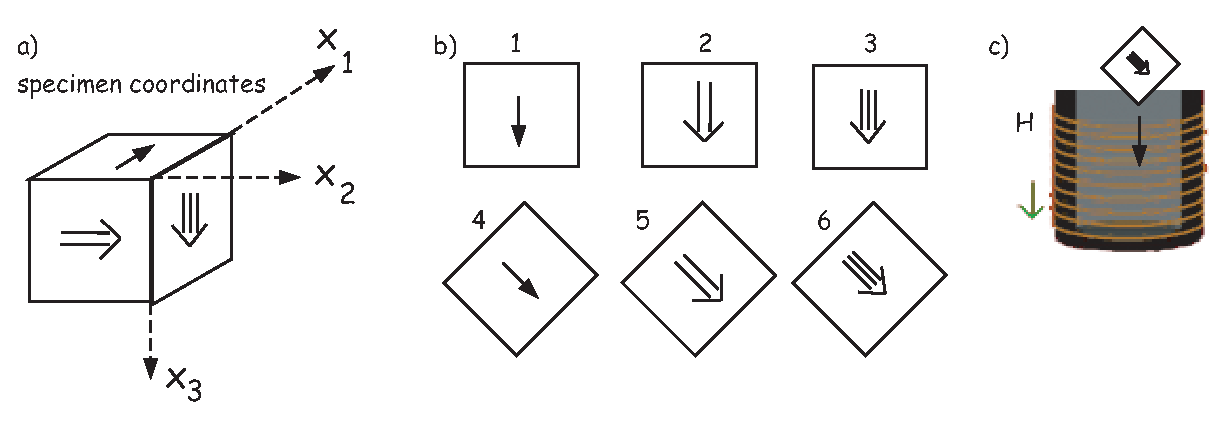
\includegraphics[width=14 cm]{EPSfiles/measAMS.eps}
\caption{Definition of specimen coordinate system.  b) Six measurement scheme for determining the anisotropy ellipsoid.  c) Position of the specimen in the magnetic smagusceptibility meter. }
\label{fig:measAMS}
\end{figure}


\section{Anisotropy of magnetic susceptibility}
\label{sect:chimeas}


The relationship between a small applied magnetic field 
vector ${\H}$ and the
induced  magnetization vector ${\M}$ is the 
\index{magnetic!susceptibility!anisotropy}
 \index{anisotropy!magnetic susceptibility}
magnetic susceptibility (Chapter 1).  This relationship has until this chapter been treated  as a scalar property, independent of the directions of the field or magnetization vectors.    While isotropy is frequently an adequate approximation,  if the magnetic response of the specimen depends on the orientation of the applied field (i.e., it is anisotropic)  the response is more appropriately  approximated by a set of linear equations. 
 Components  of the induced  magnetization($\M_i$)
 in a given coordinate system  whose axes are denoted by
 $\X_1, \X_2$, and $\X_3$ (see Figure~\ref{fig:measAMS}a) relate to the components of the applied field along the specimen axes $\H_i$ 
by the following linear equations:

\begin{equation} 
\matrix{
{M}_1 =  {\chi}_{11} {H}_1 + {\chi}_{12} {H}_2 + {\chi}_{13}
{H}_3\cr
{M}_2 =  {\chi}_{21} {H}_1 + {\chi}_{22} {H}_2 + {\chi}_{23}
{H}_3\cr
{M}_3 =  {\chi}_{31} {H}_1 + {\chi}_{32} {H}_2 + {\chi}_{33}
{H}_3,\cr
}
\label{eq:MkH}
\end{equation}

\noindent where $\chi_{ij}$ are coefficients of the magnetic  susceptibility tensor.


  We have met tensors before in the orientation matrix and rotation matrices (see Appendix~\ref{app:tensors}.)   The coefficients ${\chi_{ij}}$ are the elements of a 
second-order, symmetric tensor, 
 known as the 
 \index{magnetic!susceptibility!anisotropy}
 \index{anisotropy!magnetic susceptibility}
 {\it anisotropy of magnetic  susceptibility}  (AMS) tensor
${\bf \chi}$.
The set of Equations~\ref{eq:MkH} can be rewritten in summation notation as:

\begin{equation}
M_i=\chi_{ij}H_j.
\label{eq:chi1}
\end{equation}

The susceptibility tensor ${\bf  \chi}$   has 6 independent matrix
elements because $\chi_{ij}=\chi_{ji}$. For convenience we define a column matrix $\s$ having six
elements that are related to the elements of ${\bf \chi}$ by:

\begin{equation}
\matrix
{s_1 = \chi_{11}\cr
s_2 = \chi_{22}\cr
s_3 = \chi_{33}\cr
s_4 = \chi_{12}=\chi_{21}\cr
s_5 = \chi_{23}=\chi_{32}\cr
s_6 = \chi_{13}=\chi_{31}.\cr}
\label{eq:kj}
\end{equation}

\noindent In practice, only $s_1, s_2$, and $s_3$ can be  measured directly,  the terms
$s_4$ to $s_6$ are only indirectly determined.
 In the simplest experiment, there are six measured values of  susceptibility $K_i$ made  in six  special positions.  There are many measurement schemes possible; one is  shown in Figure~\ref{fig:measAMS}b. 
Measurement in position 1 gives $K_{1}=s_1$. Similarly, in position 2, we measure 
$K_2=s_2$, and in position 3, we get $K_3= s_{3}$.  But, 
$K_4 = \half (s_{1}+s_{2}) + s_{4}$, $K_5 =  \half (s_{2}+s_{3})
+ s_{5}$, and $K_6 =  \half (s_{1}+s_{3}) + s_{6}$.
 From this we see that the  elements of
$\s$ are related to  the matrix of measurements  $\K$ in subscript notation by:
\begin{equation}
K_i = A_{ij}s_j,
\label{eq:ak}
\end{equation}
\noindent where $\A$ depends on the experimental design and is called the
{\it design matrix}.  The measurement scheme shown in   Figure~\ref{fig:measAMS}b, has the design matrix: 

\begin{equation}
\A=\pmatrix{
1&0&0&0&0&0\cr
0&1&0&0&0&0\cr
0&0&1&0&0&0\cr
.5&.5&0&1&0&0\cr
0&.5&.5&0&1&0\cr
.5&0&.5&0&0&1}.
\label{eq:a66}
\end{equation}

\noindent 
In order to calculate the best-fit values 
$\bars $ for the measurements, we can use linear algebra:

\begin{equation}
\bar s = 
(\A^T\A)^{-1}\A^T \K \hskip 1em \hbox{or} \hskip 1em \bars = \B \K,
\label{eq:bk}
\end{equation}
\noindent where  $\A^T$ is the transpose of $\A$ and $\B = (\A^T\A)^{-1}\A^T$.  
The elements of $\B$ for the scheme shown in Figure~\ref{fig:measAMS}b are readily determined as:
\begin{equation}	
\B=\pmatrix{
1&0&0&0&0&0\cr
0&1&0&0&0&0\cr
0&0&1&0&0&0\cr
-.5&-.5&0&1&0&0\cr
0&-.5&-.5&0&1&0\cr
-.5&0&-.5&0&0&1\cr}.
\label{eq:b66}
\end{equation}

\noindent In the special case in which $\A$ is a square matrix (as in
Equation~\ref{eq:a66}), $(\A^T\A)^{-1}\A^T$ reduces to $\A^{-1}$ (i.e.
$\B = \A^{-1}$). 


There exists one coordinate system $\V$ (whose axes  are the
\index{eigenvectors}
eigenvectors of ${\bf  \chi}$:
$\V_1$, $\V_2$, $\V_3$) in which the off-axis terms of ${\bf \chi}$ 
are zero (see Appendix~\ref{app:eigen}). While the eigenvectors collectively are called the ``principal axes'', the first eigenvector is also known simply as the principal eigenvector and the other two  are the major and minor eigenvector respectively.   In this special coordinate system:

\begin{equation}
\matrix{
{M}_1 =  {s}_{1} {H}_1 = \chi_{11} {H_1} \propto \tau_1 {H}_1\cr 
{M}_2 =   {s}_{2} {H}_2= \chi_{22} {H_1}  \propto \tau_2 {H}_2 \cr
{M}_3 =  {s}_{3}{H}_3= \chi_{33} {H_3}  \propto \tau_3 {H}_3. \cr}
\label{eq:MHeig}
\end{equation}

 \noindent The 
 \index{eigenvalues}
 eigenvalues $\tau_1$, $\tau_2$ and  $\tau_3$  
correspond to the  maximum, intermediate, and minimum
 susceptibility, respectively.  These are the susceptibilities  
along the principal, major and
minor eigenvectors $\V_1$, $\V_2$, and $\V_3$, respectively.
Scaling ${\bf \chi}$ by its trace yields values for ${\bf  \tau}$
that sum to unity. [Note that $\V_1,\V_2$ and $\V_3$ are sometimes referred to as $K_{max}, K_{int}$, and $K_{min}$, respectively in the literature. Also some practitioners prefer to normalize the eigenvalues such that their average is unity and not their sum.]    



\begin{figure}
%\centering \epsffile{EPSfiles/magnitude.eps}
\centering  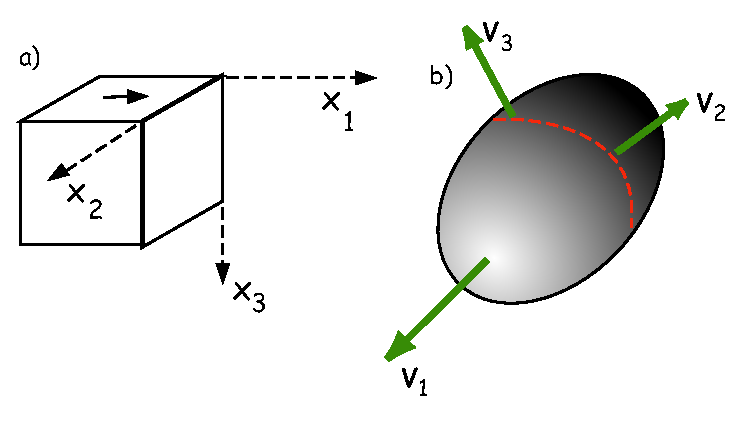
\includegraphics{EPSfiles/magnitude.eps}
\caption {a) Arbitrary coordinate system of a specimen.  b) The magnitude ellipsoid  of  AMS.   Its coordinate
system  is defined by the eigenvectors $\V_i$.  The lengths  along the eigenvectors of the ellipsoid surface are related to the eigenvalues $\tau_i$ (see text). }
\label{fig:magnitude}
\end{figure}



When the coordinate system of the susceptibility data is defined by the eigenvectors,
then the components of magnetization $M_i$ satisfy the following:

 \beq
{{M_1^2}\over{\tau_1^2}} +
{{M_2^2}\over{\tau_2^2}}+
{{M_3^2}\over{\tau_3^2}}= 1.
\label{eq:magnitude}
\eeq

The surface described by
Equation~\ref{eq:magnitude} illustrated 
in Figure~\ref{fig:magnitude}b traces an ellipsoid termed 
the 
\index{magnitude ellipsoid}
{\it magnitude ellipsoid} by  
\index{Nye, J.F.}
Nye (1957)\nocite{nye57}
 whose semi-axes are directed along the  $\V_i$  and whose lengths
are proportional to the $\tau_i$.  We will refer to
this ellipsoid in the following as the 
\index{anisotropy!ellipsoid}
anisotropy of magnetic susceptibilty
(AMS) ellipsoid.   Because it is possible to have negative eigenvalues making the magnitude ellipsoid difficult to visualize, some workers prefer the representation quadric, which has a less direct relationship to the eigenvalues.  In the case of negative eigenvalues (say for a carbonate dominated system), it is also possible to simply offset the eigenvalues by some DC offset to ensure positivity.  

Many publications list AMS data in terms of the eigenvalues and eigenvectors,
(the eigenparameters)  so it is handy to have a way to transform eigenparameters back into matrix elements.  This can be 
done using tricks from linear algebra:

\begin{equation}
{{\bf \chi}= \V {\bf  \tau} \V}^T,
\label{eq:eigsdj} 
\end{equation}

\noindent where $\V^T$ is the transpose of $\V$.   [Note that several (maybe even three) decimal places are required to do this inversion  in a satisfactory fashion, yet almost no one reports to this degree of precision and the tensor elements you get back out may be very different from those that went in if there is insufficient precision.] 


The eigenparameters of the
susceptibility tensor are related to the statistical alignment of dia-,
para-, and/or ferromagnetic
phases within the rock and the AMS ellipsoid 
can be used to describe the magnetic fabric of the rock. The eigenvectors describe the 
\index{anisotropy!ellipsoid!orientation}
orientation of the ellipsoid while the eigenvalues describe the shape. 
 Much of the interpretation of 
AMS data  in the literature revolves around an assessment of
 directions of principal axes and relative magnitudes of the eigenvalues.  

\index{anisotropy!ellipsoid!shape}
There is a bewildering variety of conventions for describing the
relationships among the three eigenvalues (see,  Table
~\ref{table:params} for a partial list).  A practical initial classification
scheme can be made with the following 
rules: when $(\tau_1 \simeq \tau_2 \simeq \tau_3)$, the shape of the ellipsoid is a sphere; when $(\tau_1
 \simeq \tau_2 >
\tau_3)$, it is oblate.  The shape is prolate when $(\tau_1 > 
\tau_2 \simeq \tau_3)$, and, finally, the anisotropy ellipsoid is triaxial
when  $(\tau_1 > \tau_2 > \tau_3)$.  Because there are nearly always
three distinct values of $\tau$,  
it is a statistical problem to decide whether
the eigenvalues from a given data set are significantly different 
from one another.

Making only six measurements allows calculation of the
eigenparameters, but gives no constraints for their uncertainties.  
We would like to ask questions such as the following:

\begin {quote}
1)  Is a particular axis parallel to some direction? 
Is $\V_3$  vertical as might be expected for a primary sedimentary fabric?
Is $\V_1$ parallel to some lineation such as elongated
vesicles in volcanic dikes, or deformed ooids in strained rocks?

2) Are two sets of eigenvectors distinct?  Are data
from two sides of a dike margin imbricated, allowing interpretation of
flow direction? Has progressive strain rotated the rock fabrics?

3) What is the shape of the AMS ellipsoid? Are the eigenvalues distinct?
Is the fabric oblate, as for  consolidated, undeformed sedimentary rocks?  Does the shape
change as a result of progressive deformation in metamorphic rocks? 

\end{quote}


In order to address questions such as these,
 we need some sort of confidence intervals
for the eigenparameters; hence we need to make 
more than six measurements and we need a 
means of translating the measurements into uncertainties in AMS data.  
The principles of error analysis for anisotropy measurements were originally
laid out by
\index{Hext, G.R.}
  Hext (1963),   \nocite{hext63}  and were later fleshed out by 
  \index{Jelinek, V.}
  Jelinek (1978).  \nocite{jelinek78}  These are analytical approaches.  \index{Constable, C.G.}
\index{Tauxe, L.}
Constable and Tauxe (1990) \nocite{constable90}
took an entirely different approach using a bootstrap.  We will begin with the 
\index{Hext, G.R.}
Hext (1963) \nocite{hext63}
method which serves as the foundation for all modern AMS statistical analysis.  

\index{Hext!statistics}
\section{Hext Statistics}
\label{sect:hext}

Each measurement $K_i$ has an unknown
measurement uncertainty $\delta$ so we can write:  

\begin{equation}
K_i = A_{ij}s_j + \delta_i.
\label{eq:kdel}
\end{equation}

\noindent
Hext (1963) defined  the residual sum of squares $S_o$ to be:
\begin{equation}
S_o= \sum_i \delta_i^2 , 
\label{eq:So}
\end{equation}

and the estimated variance $\sigma^2$ as:
\begin{equation}
\sigma^2=S_o/n_f.
\label{eq:s2}
\end{equation}
\noindent $n_f$ is the number of degrees of freedom, given
by $N_{meas}-6$ where $N_{meas}$ is the number of measurements and six is the minimum number of measurements required to determine the susceptibility tensor.  


\begin{figure} [htb]
%\epsfysize 3in
%\centering \epsffile{EPSfiles/eij.eps}
\centering  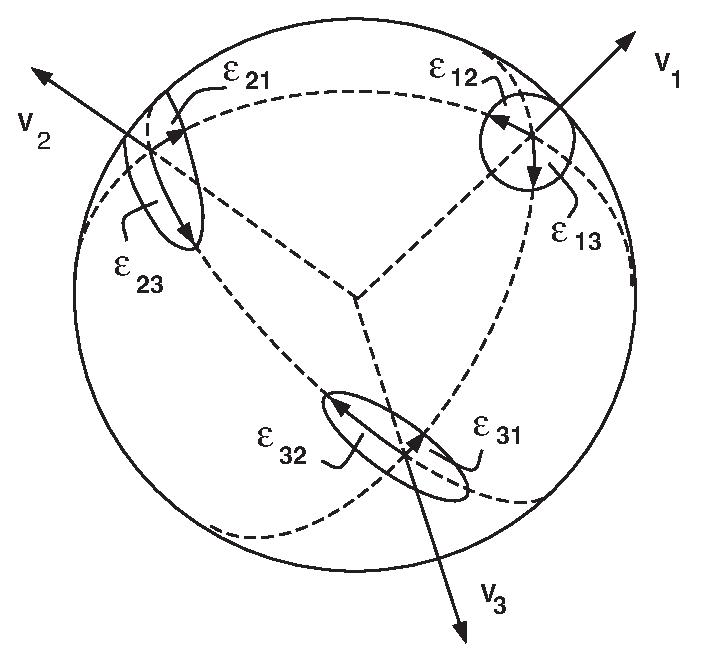
\includegraphics[width=3 in]{EPSfiles/eij.eps}
\caption
{Relationship of the uncertainty ellipses (calculated by Hext statistics for AMS 
data) to the principal axes. The major and minor semi-axes of the
 uncertainty ellipses are oriented along the axes defined by the
eigenvectors. [Figure from Tauxe, 1998.] }
\label{fig:eij}
\end{figure}
\nocite{tauxe98}


\index{anisotropy!magnetic susceptibility!measurement of}
There are  many measurement schemes in common usage with as few as six (for which  $\sigma^2$ is undefined)  and as many as several hundred.    The scheme of 
  \index{Jelinek, V.}
  Jelinek (1976), has  $N_{meas}$ = 15, and  is described in detail in Appendix~\ref{app:K15}.   Spinning susceptibility meters have more recently been introduced that measure magnetic susceptibility as the specimen spins around each of three axes (see Figure~\ref{fig:AMSspin}).   
The procedure used in the SIO lab (see e.g., 
\index{Gee, J.S.}
Gee et al., 2008
 \nocite{gee08} 
for details) is also briefly described in Appendix~\ref{app:AMSspin}.  

Each measurement system has an associated design matrix from which the $\B$ matrix of Equation~\ref{eq:bk} can be determined.     Once the $\B$ matrix  is set up,  we can calculate 
the best-fit values for
$\s$:
\begin{equation}
\bar s_i = B_{ij} K_j.
\label{eq:barchi}
\end{equation}

\noindent The best-fit values for $\K$ ($\barK$) 
can then be calculated by substituting the right $\A$ matrix (see e.g., Appendix~\ref{app:K15}): 
$$
\bar K_i = A_{ij}\bar s_j.
$$
\noindent
Now we can calculate the $\delta_i$ by:
\begin{equation}
\delta_i = K_i-\bar K_i,
\label{eq:deli}
\end{equation}

\noindent and $S_o$ is given by Equation~\ref{eq:So}. 

Assuming that the uncertainties in $\K$ (the $\delta_i$)
 have zero mean, and that they are uncorrelated, normally
distributed, and small (so that the products of uncertainties can
be neglected),  Hext (1963) proposed that approximate 95\% confidence
ellipses for the eigenvectors (see Figure~\ref{fig:eij}) can  be calculated as described as follows:

\index{Hext!confidence ellipses}
\subsection{Hext confidence ellipses}
\label{sect:hextE}

The Hext (1963) confidence ellipses shown in Figure~\ref{fig:eij} are calculated as follows: 

\begin {enumerate}

\item We assume that the uncertainties in the eigenvectors
 are in a plane that is tangent to the unit sphere.  We
further assume that they belong to a two-dimensional normal
distribution with semi-axes that are aligned along the $\V_i$.  The ellipse
with semi-axes $\epsilon_{ij}$ that
outline a 95\% confidence region in this plane is then projected onto the
sphere  (Figure~\ref{fig:eij}). 

\item Calculate the matrices $\bars$, $\barK$, and the
$\delta_i$ from the
measured values of $\K$.

\item Calculate the eigenvectors  $\V$ and eigenvalues
${\bf  \tau}$ of $\bars$.

\item  Calculate $\sigma$ by Equations~\ref{eq:So} and \ref{eq:s2}.

\item The confidence regions are outlined by ellipses along
semi-axes $\epsilon_{ij}$ aligned with the eigenvectors.
The $i$ subscripts refer to the axis on which
the ellipse is attached and the $j$ subscripts refer to the axis to which it
points. Thus, $\epsilon_{12}$ is the semi-axis that defines the confidence
region of $\V_1$ directed toward $\V_2$ (Figure~\ref{fig:eij}).

The three unique semi-angles of the confidence ellipses 
$\epsilon_{ij}$ are calculated by:

\begin{equation}
\matrix
{\epsilon_{12}= \tan^{-1}[f \sigma/2(\tau_1-\tau_2)]\cr
\epsilon_{23}= \tan^{-1} [f \sigma/2(\tau_2-\tau_3)]\cr
\epsilon_{13}= \tan^{-1} [f \sigma/2(\tau_1-\tau_3)]\cr
\epsilon_{21}=\epsilon_{12}\cr
\epsilon_{32}=\epsilon_{23}\cr
\epsilon_{31}=\epsilon_{13},\cr
}
\label{eq:eij}
\end{equation}

\noindent where

$$
f=\sqrt{ 
{2(F_{(2,n_f);(1-p)})},
}
$$

\noindent and  where $F_{(2,n_f)}$ is the value from the $F$ table (see F-tables in a statistics book or online), with 2 and
$n_f$ degrees of freedom, at the $p$ probability level.  The
value of $F_{(2,n_f)}$ for $N_{meas} =15$ measurements ($n_f=9$) at the 95\% level of
confidence ($p=.05$) is 4.26 and so $f$ = 2.92.
\end {enumerate}

\index{statistical tests!Hext's F tests}
\subsection{Hext $F$ statistics for significance of eigenvalue ratios}


Because of the  mindless precision of modern computers, there are always three different eigenvalues returned by subroutines for eigenparameter calculation.  But, these may not be significantly different from one another.  In order to test for significance, Hext (1963) developed three $F$ statistics:  $F$ for significance of overall anisotropy, $F_{12}$ for significant difference between the maximum and intermediate eigenvalues  (are the data oblate?) and $F_{23}$ for significant difference between the intermediate and minimum eigenvalues (are the data prolate?).  (If all three are positive, the data are triaxial).  The $F$ statistics are calculated as follows:

\begin{equation}
\matrix{
F = 0.4 (\tau_1^2 + \tau_2^2 + \tau_3^2 - 3\chi_b^2)/\sigma^2\cr
F_{12} = 0.5((\tau_1 - \tau_2)/\sigma)^2\cr
F_{23}= 0.5((\tau_2 - \tau_3)/\sigma)^2,\cr}
\label{eq:fij}
\end{equation}
 \noindent where the bulk susceptibility $ \chi_b $ 
is given by:
\begin{equation}
\chi_b = (\bar s_1+\bar s_2+\bar s_3)/3.
\label{eq:chib}
\end{equation}


The critical value for $F$ (when $N_{meas}$ = 15)  is 3.4817 for 95\% confidence  (for $F_{12}$ and  $F_{23}$, it is 4.2565). 
So, we can test  if the data are isotropic ($F$)
$(\tau_1=\tau_2=\tau_3)$, if
$\tau_1 = \tau_2$ ($F_{12}$), or if $\tau_2=\tau_3$ ($F_{23}$).
 $F$ values below the critical
values do not allow rejection of the null  hypotheses of isotropy or
rotational symmetry, respectively.  





\section {Limitations of  Hext statistics}

The assumptions for using 
\index{Hext!statistics}
Hext statistics (Section~\ref{sect:hext}) are
that the uncertainties in the measurements have zero mean, are
normally distributed, and are small.  While measurement error using modern
equipment 
is likely to be quite small,
data from a collection of specimens often do not conform to these
restrictive assumptions.  In particular, the $\delta$ values
are often large.

\index{Constable, C.G.}
\index{Tauxe, L.}
Constable and Tauxe (1990)
showed that, in general, $\delta$s from AMS data calculated for
 multiple specimens (that must be normalized by their trace) will not 
 be normally distributed.  Hence, data incorporating multiple specimens
 are often not amenable to Hext statistics.   For this reason, Constable and Tauxe (1990) developed a 
 \index{bootstrap!anisotropy tensors}
 bootstrap for  paleomagnetic tensors.  Their bootstrap was developed for  AMS data but anisotropy of remanence data could be treated in a similar manner.  

\section {Bootstrap confidence ellipses}



\begin{figure} [htb]
%\epsfxsize 14cm
%\centering \epsffile{EPSfiles/evec.eps}%data from tr213
\centering  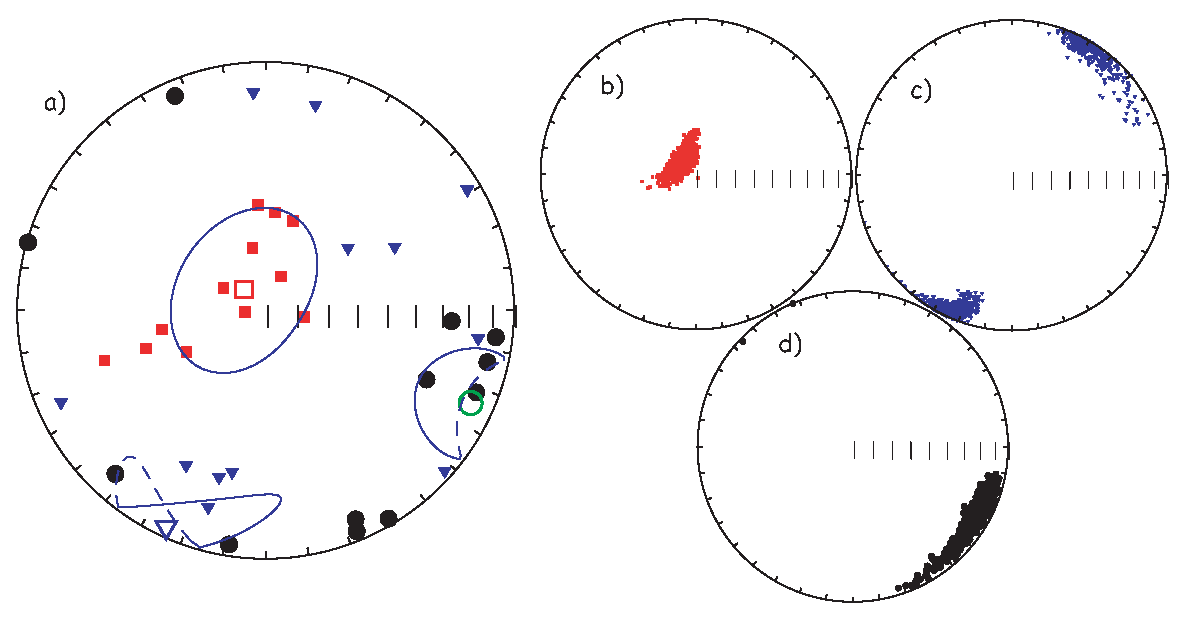
\includegraphics[width=14 cm]{EPSfiles/evec.eps}
\caption{
a) Lower hemisphere projection of directions of
 $\V_1$ (squares), $\V_2$ (triangles), and $\V_3$ (circles) from the 
margin of a volcanic dike.   Open symbols are the Hext means.  Thin blue lines are the Hext 95\% confidence ellipses (dashed portion are on the upper hemisphere).  
b) Equal area projection of  principal eigenvectors 
($\V_1$)  of 500 pseudo-samples drawn from the data in a). c) Same as b) for the 
major eigenvectors  ($\V_2$).
d) Same as b) for the minor eigenvectors ($\V_3$).  [Data from Tauxe et al., 1998.]}
\label{fig:evec}
\end{figure}
\nocite{tauxe98b}

To motivate the discussion of statistical analysis of AMS data, we will use a data set collected from the margins of dikes from the ophiolite sequence exposed on the Island of Cyprus (data from 
\index{Tauxe, L.}
Tauxe et al. 1998).
\nocite{tauxe98b} 
% [These samples were collected during a project inspired by the work of Knight and Walker (1988)  in which we tried to use AMS data to determine the direction of magma flow within the dikes (e.g., Staudigel et al. 1992).] \nocite{staudigel92}  
The eigenvectors  in Figure~\ref{fig:evec}a  are those estimated for individually oriented samples from one of the quenched margins of a dike.  They are plotted on an equal area projection following the convention of 
lower hemisphere projections with the $\V_1$s as squares, $\V_2$s as triangles,
and $\V_3$s as circles. Open symbols are the mean values.  
The data are rather typical for those obtained  from a single 
homogeneous body of rock  in that the  $\delta$ distributions are neither 
normally distributed, nor
small.  

The Hext 95\% confidence ellipses are shown as thin blue lines (dashed on the upper hemisphere.    The confidence ellipses for the maxima (squares) and intermediate (triangles) eigenvectors follow the trends in the data, but that for the minima (circles) does not.  In fact the ellipse for the minimum axis appears to be orthogonal to the trend in the data.   It also seems that the confidence ellipses are quite large and at least for the maximum eigenvector, too wide.      The problem with Hext statistics is that it is only suitable for data sets with small $\delta_i$ that are normally distributed.  


 In order to deal with data that do not fit the requirements for Hext statistics, 
 \index{Constable, C.G.}
 \index{Tauxe, L.}
 Constable and Tauxe (1990) 
developed a bootstrap for anisotropy data,  similar to that introduced in Chapter 12 for vectors.  We take a number of randomly selected pseudo-samples  and calculate the Hext  average   $\bar s$ matrices and their eigenparameters.  The bootstrapped eigenvectors are shown    in Figure~\ref{fig:evec}(b-d). 

A non-parametric confidence region for the bootstrapped distributions
 shown in Figure~\ref{fig:evec}b-d could  be drawn as 
a contour line enclosing 95\% of the bootstrapped eigenvectors.  
Because it is often useful to characterize the average uncertainties with
a few parameters (for example, to put them in a data table),
 we can proceed as with the unit vectors and assume
some sort of distribution for the eigenvectors, for example,  the Kent distribution from Chapter 12).  However, for most of the questions outlined
at the beginning of the chapter, it is preferable to assess directly  the 
95\% confidence bounds on the parameter of interest.


By analogy with  the bootstrap for unit vectors and the 
fold test, we can also
perform  parametric bootstraps.  There are two flavors of these:  the {\it specimen parametric bootstrap} and the {\it site parametric bootstrap}.  For the specimen parametric bootstrap,  proceed as follows:
After randomly selecting
a particular specimen for inclusion, each element $\s_i$ is replaced by a
simulated element drawn from a normal distribution having a mean of $\s_i$ and 
$\sigma$ as calculated for the specimen.
This Monte Carlo type simulation  assumes
that the measurement uncertainties are normally distributed, which 
 is likely to be the case.  If instrument noise is significant, then
the specimen parametric bootstrap can be an important tool. 


Because the $\delta_i$ data from homogeneous rock bodies are often normally 
distributed (although not necessarily small), we can also perform a parametric bootstrap at the level of
the site (the {site parametric bootstrap}).  This is done by drawing pseudo-samples 
as before, but replacing individual elements of $\s_i$ with simulated data
drawn from normal distributions with mean of $\s_i$, but using the standard deviation 
calculated from the data for an entire site.  
This procedure goes a long way
toward estimating realistic confidence intervals from sites with too few
specimens.  

Speaking of ``too few samples'',  it is important to  emphasize again that bootstrapped confidence ellipses are only asymptotically correct, relying on the assumption that the full statistical variability is represented in the data set.  It is inadvisable to rely on bootstrapped uncertainties with fewer than about 20 specimens as they will be too small.  If it is possible to perform a parametric bootstrap (i.e., the $\delta$s are normally distributed), then perhaps as few as six specimens can be done (see 
\index{Tauxe, L.}
Tauxe et al. 1998 for a more complete discussion).  \nocite{tauxe98b}     


\begin{figure}[h!tb]
%\epsfxsize 13cm
%\centering \epsffile{EPSfiles/kmin.eps}
\centering  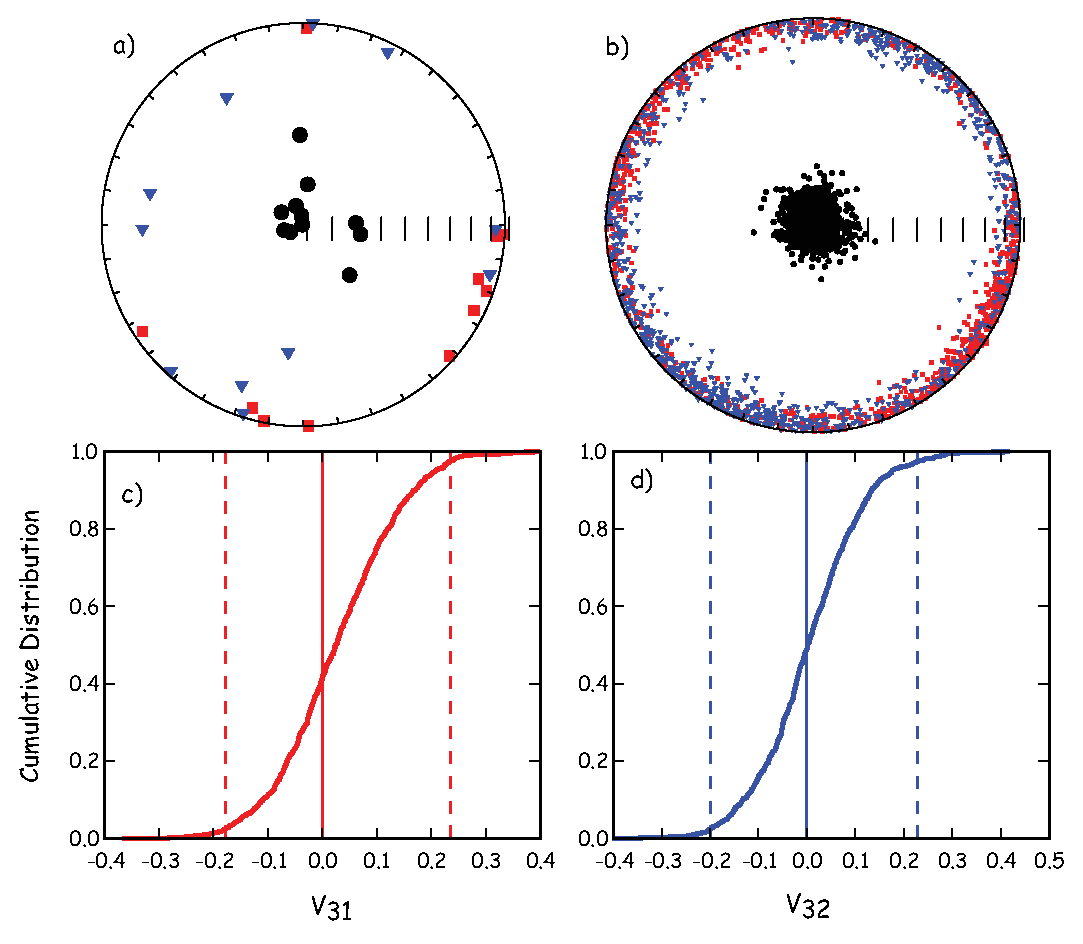
\includegraphics[width=13 cm]{EPSfiles/kmin.eps}
\caption{a) AMS data from Cretaceous carbonate limestones in Italy (the
Scaglia Bianca Formation) in tilt adjusted coordinates. a) Lower
hemisphere projections of the principal $\V_1$ (squares), major 
$\V_2$ (triangles), and minor $\V_3$ (circles) eigenvectors.  
b) Bootstrapped eigenvectors
from pseudo-samples of the data in a).  c) Cumulative distribution of the $v_{31}$ with bounds containing 95\% of the components plotted as dashed lines.
The zero value expected from a vertical direction is shown as a 
vertical solid line.  d) Same as c) but for the $v_{32}$ components. [Data from Cronin et al., 2001.] }
\label{fig:kmin}
\end{figure}
\nocite{cronin01}

\section{Comparing mean eigenvectors with other axes}

We can now  consider whether a particular axis is distinct from
a given direction or another eigenvector.  For example, we may wish to know
if a given data set from a series of sediments has a vertical minor 
eigenvector as would be expected for a primary sedimentary fabric.  
In Figure~\ref{fig:kmin}a we show AMS data from samples taken 
from the Scaglia Bianca Formation (Cretaceous white limestones)
in the Umbrian Alps of Italy.  They have been rotated into  tilt adjusted 
coordinates; hence the bedding pole is vertical.
Instead of plotting the 95\% confidence ellipses, which all require
 unnecessary parametric assumptions, we show the bootstrap eigenvectors in 
Figure~\ref{fig:kmin}b.  The smear of points certainly covers the vertical
direction,  consistent with a  vertical direction for $\V_3$.  To
make the test at a given level of confidence (say 95\%), we can employ the
method developed for unit vectors in which the set of bootstrapped vectors for the eigenvector of
choice (here $\V_3$) are converted to cartesian coordinates,  sorted and plotted as a cumulative distribution (see  Figure~\ref{fig:kmin}c and d).
\index{bootstrap!eigenvectors}%
Now the bootstrapped
 95\% confidence bounds can be directly compared with the expected
value.  For a direction to be vertical, both the $x_1$ and $x_2$ components
must be indistinguishable from zero (see solid line in the figure).  Because zero is included within
the confidence intervals in Figures~\ref{fig:kmin}c and d respectively, the  data  shown in Figure~\ref{fig:kmin}a have a minor eigenvector axis  that cannot be distinguished from vertical 
 at the 95\% level of confidence.
 




Another question that often arises is whether eigenvectors from  
two sets of anisotropy data can be 
distinguished from one another. For example, are the $\V_1$ directions from data sets
collected from two margins of a dike different from one another and on opposite
sides of the dike plane as expected from anisotropy controlled by silicate
imbrication.  



\begin{figure}[htb]
%\epsfxsize 12cm
%\centering \epsffile{EPSfiles/dikeams.eps}
\centering  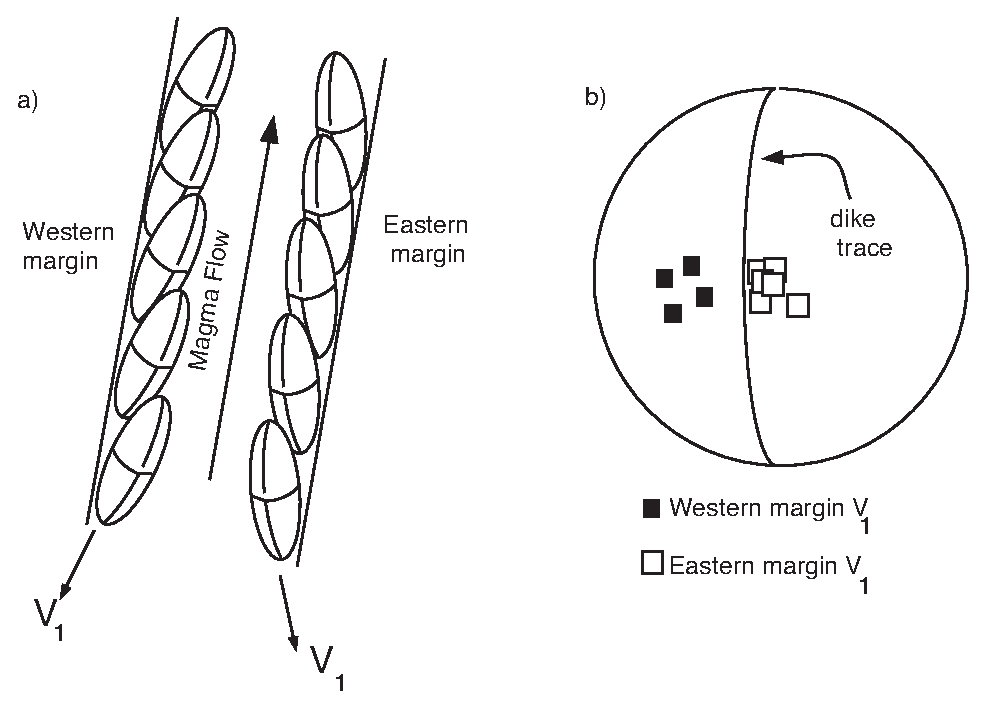
\includegraphics[width=12 cm]{EPSfiles/dikeams.eps}
\caption{Principles of AMS for interpretation of flow directions in dikes. [Figure from Tauxe, 1998 after 
Knight and Walker, 1988; ]}
\label{fig:dikeams}
\end{figure} \nocite{knight88,tauxe98} 

The principles by which flow directions can be determined in volcanic dikes
were laid out by  
\index{Knight, M.D.}
\index{Walker, G.P.L.}
Knight and Walker (1988). \nocite{knight88} 
While the magma is flowing in the
dike, elongate particles 
 become imbricated against the chilled margins (see Figure~\ref{fig:dikeams}).
Opaque phases such as magnetite are often observed to be 
distributed along the fabric of 
the silicate phases (see 
\index{Hargraves, R.B.}
 Hargraves, 1991).\nocite{hargraves91} 
The principal eigenvectors arising from such a
{\it distribution anisotropy} parallel the  fabric of the silicates.
 In Figure~\ref{fig:dikeams}b,
we show that in the ideal case,
the $\V_1$ directions from the two margins are distinct and 
fall on either side of the dike trace.  Because the convention is to plot AMS
data in lower hemisphere projections, the fact that the western margin data
plot on the western side, and the eastern margin data plot on the eastern side
suggests that the flow was upward.  Thus, the AMS data from 
chilled margins of dikes can give not only a lineation, but a well constrained
direction of magma flow. 


Some of the earliest magnetic measurements made on sediments were of
anisotropy of magnetic susceptibility (see summary by 
\index{Tarling, D.H.}
\index{Hrouda, F.}
Tarling and Hrouda, 1993). \nocite{tarling93} In general, these data   show that
 the  magnetic fabric of sediments is strongly
affected by the depositional environment  (see Figure~\ref{fig:sedams}). 
For example, quiet water deposition ( Figure~\ref{fig:sedams}a) should have $\V_3$ directions that are  perpendicular to the bedding plane, with  an oblate AMS ellipsoid.
 In moderate currents (no particle entrainment) (see Figure~\ref{fig:sedams}b),  particles should be imbricated, resulting in (slightly) off-vertical $\V_3$
directions.    The $\V_1$ direction (in lower hemisphere projections)
is antiparallel to the paleo-flow direction,  and the fabric is characterized by an oblate AMS ellipsoid.  But when deposition occurs under high current flow (with particles entrained) (Figure~\ref{fig:sedams}c), the $\V_3$ distribution should be streaked.     $\V_1$ should be perpendicular to  the flow direction, and
the fabric is characterized by prolate or triaxial AMS ellipsoids.     Each of these categories relies on some assessment of shape but the data may not be suitable for Hext statistics.   We therefore require some non-parametric (bootstrap) way of characterizing the basic shapes in anisotropy ellipsoids.  



\begin{figure}[htb]
%\epsfxsize 12cm
%\centering \epsffile{EPSfiles/sedams.eps}
\centering  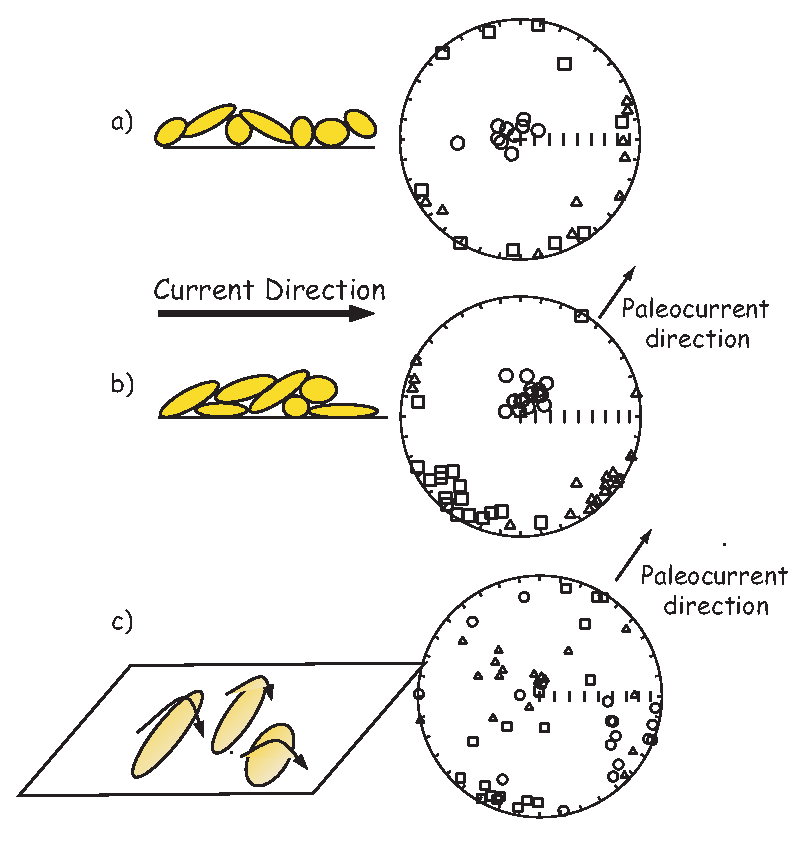
\includegraphics[width=12 cm]{EPSfiles/sedams.eps}
\caption{Characteristics of AMS data from sediments deposited in
a) quiet water, b) moderate water flow, and c) flow that is
sufficient to entrain particles.  [Figure adapted from Tauxe, 1998.]
 }
\label{fig:sedams}
\end{figure}

 
 


\begin{figure}[h!tp]
%\epsfxsize 14cm
%\centering \epsffile{EPSfiles/shape.eps} 
 \centering  \includegraphics[width=14 cm]{EPSfiles/shape.eps}
 \caption{Determination of the shape of AMS data using the bootstrap. Conventions as in Figure 13.4 a-d)  Selected data sets plotted as eigenvector directions from individual specimens.  
e-h) Bootstrapped eigenvectors from a-d) respectively.   i-l) Cumulative distributions  of the bootstrapped eigenvalues 
associated with the eigenvectors plotted in e-h).   The bounds containing 95\% of each eigenvalue are shown as vertical dashed dot line for $\tau_3$, dashed for $\tau_2$ and solid for $\tau_1$.   }
\label{fig:shape}
\end{figure}

\section {Shape}


While there  are innumerable ways of  characterizing shapes of anisotropy
ellipsoids in the literature, all discussions of ``shape'' revolve
around the relationships between the various eigenvalues. 
The first
question to consider is whether these can be distinguished in a
statistical sense. 
The $F$ parameters in Hext (1963)  statistics allow us 
 to check for significance of the difference between the eigenvalues. However, the approximations involved in the
Hext method make it inappropriate for many data sets involving more than one
sample.  Bootstrapping has  less restrictive
assumptions that allow statistical tests to be applied more widely.

Here we outline a 
\index{bootstrap!eigenvalues}
 bootstrap test for comparing two eigenvalues that is  quite similar to the bootstrap test for
common mean described in Chapter 12. In Figure~\ref{fig:shape}a-d, we
show the eigenvectors from four typical data sets.    Bootstrapped eigenvectors from these data sets   are shown in Figure~\ref{fig:shape}e-h.   In the next panel (Figures~\ref{fig:shape}i-l) , we plot cumulative distributions of the eigenvalues  along with their 95\% confidence bounds.  
   These provide a means for quantifying the shape tests defined
earlier.   For example, in 
 Figure~\ref{fig:shape}a,  the data represent an essentially spherical shape. The  three
eigenvalues plotted in the 
\index{diagrams!cumulative distribution}
cumulative distribution diagram (Figure~\ref{fig:shape}i)
have overlapping confidence intervals, hence they are
indistinguishable.  The corresponding bootstrapped eigenvectors shown 
in Figure~\ref{fig:shape}e plot in a cloud with very blurred boundaries between the minor and other eigenvector directions.  

In Figure~\ref{fig:shape}b we show data characteristic of an oblate
ellipsoid.   The
$\V_3$ eigenvector is reasonably well defined, but 
the distribution of bootstrapped $\V_2$ and $\V_1$ form a girdle 
distribution (Figure~\ref{fig:shape}f).   The defining characteristic for oblate ellipoids is that the smallest  eigenvalue is distinct from the intermediate one, while the intermediate eigenvalue is indistinguishable from the largest and this is clearly the case (see Figure~\ref{fig:shape}j).    

Data from a prolate ellipsoid are plotted in Figure~\ref{fig:shape}c.  The $\V_1$ directions are nicely defined, but the 
$\V_2$ and $\V_3$ directions are smeared in a girdle
(Figure~\ref{fig:shape}g).    The bootstrapped eigenvalue distributions  show that the 
 $\tau_1$ distribution is separate from the other two, but   $\tau_2$ and $\tau_3$ are clumped together  
(Figure~\ref{fig:shape}k).  


Finally, data from the triaxial case are shown in Figure~\ref{fig:shape}d.  The corresponding eigenvectors well grouped
(Figure~\ref{fig:shape}h) and all three
eigenvalues are distinct (Figure~\ref{fig:shape}l).   


 
There is no ``right'' way to plot eigenvalue data.  Each application requires careful thought as to what is actually being tested.  What do you want to know?  
The cumulative distribution method illustrated in Figure~\ref{fig:shape}
 is most appropriate for  classifying shape
characteristics of a relatively homogeneous set of samples.  However,  
it may not be ideal for examining trends in behavior among samples or data sets.
For example, one may wish to show the progressive change in shape and
degree of anisotropy as a function of metamorphism. In such a case, plots that boil the shape down to a single parameter may serve better.   Or one may wish to examine temporal trends in shape, for example the progressive change in sedimentary fabric with depth.  In this case, plots of eigenvalues versus stratigraphic position may be the most useful way of looking at the data.    In any case there are a plethora of anisotropy parameters in the literature.  
 We list some of the more 
popular so-called ``shape parameters'' in Table~\ref{table:params}.


Many researchers use the 
{\it total anisotropy}  parameter of 
\index{Owens, W.H.}
Owens (1974). \nocite{owens74}
This has the uncomfortable property of ranging up to 300\%; hence, we prefer
the parameter  called here the \% anisotropy of 
\index{Tauxe, L.}
Tauxe et al. (1990)\nocite{tauxe90} 
 as this
ranges from 0
 - 100\%.  The so-called ``corrected anisotropy'' of
  \index{Jelinek, V.}
  Jelinek (1981) \nocite{jelinek81}
  has several definitions in the literature (compare for example
\index{Borradaile, G.J.}
 Borradaile (1988) \nocite{borradaile88} with 
   \index{Jelinek, V.}
   Jelinek (1981); 
we have used the  original definition of Jelinek (1981).  

With the variety of shape parameters comes a host of plotting conventions.  
We will consider four types of plots here: 
the
\index{diagrams!Flinn}
Flinn diagram ($F$ versus $L$) after 
\index{Flinn, D.}
Flinn (1962), \nocite{flinn62} the 
\index{diagrams!Ramsay}
Ramsay diagram ($F'$ versus $L'$) after 
\index{Ramsay, J.G.}
 Ramsay (1967),\nocite{ramsay67}
 the 
\index{diagrams!Jelinek}
 Jelinek diagram ($P'$ versus $T$) after 
 \index{Jelinek, V.}
Jelinek 
(1981),   \nocite{jelinek81} and the
\index{diagrams!ternary}
 ternary projection (see 
 \index{Woodcock, N.H.}
Woodcock, 1977 \nocite{woodcock77}  and 
\index{Tauxe, L.}
 Tauxe et al., 1990).  The Flinn, Ramsay, and Jelinek diagrams are shown in Figure
~\ref{fig:diags} and the ternary projection is shown in Figure~\ref{fig:tern1}.  

\begin{figure}[htb]
%\epsfxsize 13cm
%\centering \epsffile{EPSfiles/diags.eps}
\centering  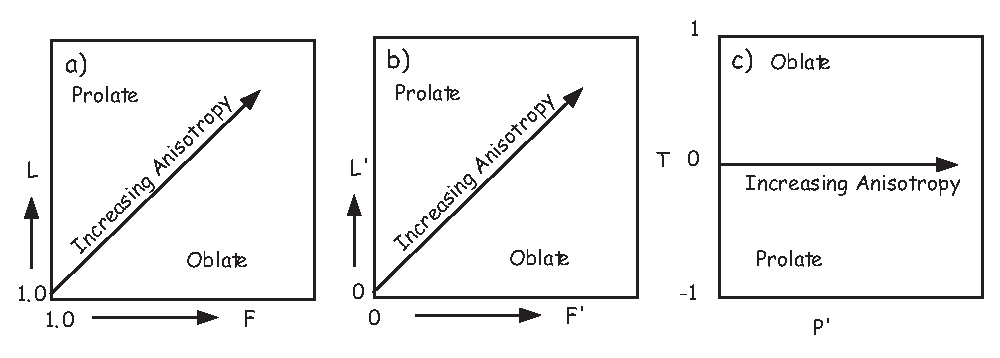
\includegraphics[width=13 cm]{EPSfiles/diags.eps}
\caption{Properties of various AMS diagrams: a) Flinn,  b) Ramsay and c)
Jelinek. [Figure from Tauxe, 1998.] }
\label{fig:diags}
\end{figure}




The Flinn and Ramsay diagrams are very similar, but the Ramsay plot has the
property of having a zero minimum as opposed to starting at 1.0 as in
the Flinn diagram.  Both are essentially polar plots, with 
radial trajectories indicating increasing anisotropy.  Shape is
reflected in the angle, with ``oblate'' shapes below the line and ``prolate''
shapes above.  

It is important to remember that, in fact, only points along the
plot axes themselves are truly
oblate or prolate and that all the area of the plot is in the ``triaxial''
region.  Because of statistical uncertainties, samples that plot in this region may fail the $F_{12}$ or $F_{23}$ tests of Hext and be classifiable as
``oblate'' or ``prolate''.  In general, however, only a narrow zone near
the axes can be considered oblate or prolate, so these terms are often
used loosely. 

   In the  Jelinek diagram  ``corrected'' anisotropy increases along the horizontal axis and shape is
reflected in the vertical axis.  There is no real advantage to using the highly
derived $P'$ and $T$ parameters over the Ramsay or Flinn plots.  Nonetheless
they are quite popular
\index{Tarling, D.H.}
\index{Hrouda, F.}
 (Tarling and Hrouda, 1993).  \nocite{tarling93}


In the ternary
projection, there are actually three axes (see Figure~\ref{fig:tern1}a).
The projection can be plotted  as a normal X-Y plot by using the $E'$ and
$R$ parameters listed in Table 1 (see Figure~\ref{fig:tern1}b).

  In none of the various types of  plots  just discussed are the
horizontal and vertical axes independent of one another, but all the
diagrams reflect the essence of the ellipsoid shape.  
Unlike the cumulative distribution plots shown in Figure~\ref{fig:shape} with bootstrap confidence intervals,
it is not possible to determine whether the
various eigenvalues or ratios thereof can be distinguished from one another
 in a statistical sense.

\begin{figure}[htb]
%\epsfxsize 12cm
%\centering \epsffile{EPSfiles/ternaryams.eps}
\centering  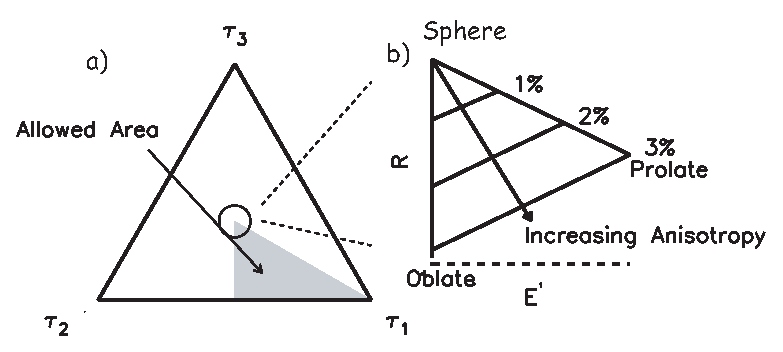
\includegraphics[width=12 cm]{EPSfiles/ternaryams.eps}
\caption{Properties of the Ternary diagram: a) There are three axes
with limits of $\tau_1,\tau_2, \tau_3$.  Because of the constraint that
$\tau_1>\tau_2>\tau_3$, only the shaded region is allowed. This is
bounded at the top by a sphere when all three eigenvalues are equal, to
the bottom left by a disk and to the bottom right by a
needle.  Geological materials generally have a low percentage of anisotropy
and plot close to the sphere.  This region is enlarged in b) which
illustrates how the ternary projection can be plotted as $E'$ versus
$R$ and how  shape (oblate, prolate, sphere) and 
percent anisotropy appear on the diagram. [Figure from Tauxe, 1998.] }
\label{fig:tern1}
\end{figure}

  




  
 
\begin{table}[htb]
\begin{center}
\caption{Assorted anisotropy statistics.}
\label{table:params}
\begin{tabular}{ll}
\hline
Parameter (Reference) & Equation\\
\hline
Bulk Susceptibility (see text) &$\chi_b=(s_1+s_2+s_3)/3$\\
Normalized eigenvalues (see text) &$\tau_1+\tau_2+\tau_3=1$\\
Log eigenvalues (Jelinek, 1981)&$\eta_1=\logn s_1; \eta_2=\logn s_2; \eta_3=\logn
\s_3$\\
Log mean susceptibility (Jelinek, 1981)&$\bar \eta=(\eta_1+\eta_2+\eta_3)/3$\\
\\
Magnitude of Anisotropy:\\
\% Anisotropy (Tauxe et al. , 1990) & $\%h = 100(\tau_1-\tau_3)$\\
 ``Total'' Anisotropy (Owens, 1974)&$A=(s_1-s_3)/\chi_b$\\
Anisotropy Degree  (Nagata, 1961)&$P=\tau_1/\tau_3$\\
``Corrected'' Anisotropy (Jelinek, 1981)&$P'=e^{\sqrt{2[(\eta_1-\bar \eta)^2 +(\eta_2-\bar \eta)^2 +(\eta_3-\bar \eta)^2}]}$ \\
\\
Shape:\\
Shape Factor (Jelinek, 1981])&$T=(2\eta_2-\eta_1-\eta_3)/(\eta_1-\eta_3)$\\
 Lineation (Balsley and Buddington, 1960)&$L=\tau_1/\tau_2$\\
Foliation  (Stacey et al., 1960)&$F=\tau_2/\tau_3$\\
 log Lineation  (Woodcock, 1977)&$L'=\logn (L)$\\
log Foliation  (Woodcock, 1977)&$F'=\logn (F)$\\
 Elongation  (Tauxe, 1998)&$E'=\tau_1+.5\tau_3$\\
 Roundness  (Tauxe, 1998)&$R=\sin(60)\tau_3$\\
\hline
\end{tabular}
\end{center}
\end{table}
 
 
\index{anisotropy!magnetic remanence}
 \section{Anisotropy of magnetic remanence}
 
 Magnetic susceptibility is somewhat like color in that many things contribute and it is often difficult to  untangle all the different contributions to tease out a meaningful interpretation.   Magnetic remanence is a much more targeted parameter because only ferromagnetic particles contribute to it and certain remanences are sensitive to only particular minerals or grain sizes.  Hence anisotropy of magnetic remanence can be a more delicate instrument than AMS.  Furthermore, certain applications such as paleointensity,  paleodirectional determinations or correction of inclination error may require the anisotropy of the TRM or DRM to be taken into account.  For example, paleointensity on pot sherds or other anisotropic specimens must be corrected for  specimen's anisotropy (e.g., 
 \index{Aitken, M.J.}
 Aitken et al. 1981) \nocite{aitken81}  and the inclination ``error'' of DRM (see Chapter 7) can be corrected using information from ARM anisotropy (e.g., 
 \index{Jackson, M.J.}
 Jackson et al. 1991).  \nocite{jackson91}
 
  ARM is often considered analogous to TRM.  Its acquisition is mathematically similar, but relies instead on variations in applied field as opposed to temperature as a blocking mechanism (see Chapter 7).   It is far more convenient to give a sample an ARM than a TRM in the laboratory, so ARM and ARM anisotropy are frequently substituted for the analogous TRM.  Of course, the two are NOT identical and proper care should be taken to ensure that the appropriate remanence is used for the particular purpose.  Nonetheless, anisotropy of ARM (AARM) is a useful measurement and we describe first how AARM is determined in the SIO laboratory.  There are slight experimental differences between AARM and ATRM which will be noted.  


 \subsection{Anisotropy of ARM and TRM}
 \label{sect:aarm}
  
 Prior to acquisition of the laboratory remanence, the specimen should be in a fully demagnetized state which is measured as a baseline.  Then one applies an  ARM  in at least three directions (say positions 1, 2 and 3 in Figure~\ref{fig:measAMS}b).   Generally, from six to 15 orientations for the ARM are used to get a reasonable estimate of the uncertainties.  [We use the nine positions 1-3, 6-8, and 11-13 in the SIO laboratory.]  Between each position, the specimen should be demagnetized along the axis of the subsequent ARM.  This measurement is  substracted from the subsequent ARM by vector subtraction.    Each  ARM step (after subtraction of the baseline)   gives  three orthogonal  remanence components    ($K^R_{ij}$).   Please note that it is possible to give ARMs in the presence of different AF fields from very high (presumably a total ARM) to lower (giving a partial ARM or pARM).  The DC field is also variable, but should be in the region where the (p)ARM is linearly related to the DC field. 
 
 The main difference between AARM and ATRM in procedure is that the demagnetization step is not required for total  TRMs.  Instead, the specimen is simply placed in each direction without the intervening baseline step.
 
 The equation for anisotropy of magnetic remanence that is analogous to  Equation~\ref{eq:MkH} is $ M_i= \chi^R_{ij} H_j $ where $\chi^R$ are the coefficients for the remanent anisotropy.     These can be reduced to the elements of $\s$ by multiplying by the appropriate $\B$ matrix, depending on the number and orientation of positions used in the experiment.  Because each measurement yields information along three axes, the design matrix has three times as many elements as for the AMS experiment with the same number of measurements.  For example, for a six position experiment, the design matrix is 18 x 6 instead of 6x6.      After determining $\s$, the other Hext parameters can be determined as before, using $n_f=3N_{meas} -6$.
 
 To correct an observed remanence vector ($\M_{obs}$) obtained through the measurement procedures outlined in Chapters 9 and 10 (direction and intensity) for the effects of anisotropy, 
 \index{Selkin, P.}
 Selkin et al. (2000b) 
 \nocite{selkin00b} 
 used  the TRM anisotropy tensor (or ARM tensor) $\chi_R$ as follows.  
 
 The ancient field direction $\H$ is given by:
 
 $$
 \H_{anc}= \M \cdot {\chi_R}^{-1}. 
 $$

\noindent To get an anisotropy corrected intensity ($|M_{AC}|$), however, we must multiply the magnitude of the observed vector $\M$ by the ratio of the magnetization acquired in a unit field applied along the lab field direction  ($\M_l = \chi_R \cdot  { \H_{lab}}$)  with that acquired in a unit field applied along the ancient field direction ($\M_a=\chi_R \cdot {\H_{anc}}$):

$$
|\M_{AC}| =  |\M_{obs}| \cdot {  {|\M_a|} \over {|\M_l|} }.
$$
 
 \subsection{Anisotropy of DRM}
 
Inclination of DRM is often too shallow (see Chapter 7) and  laboratory experiments show that it follows a tangent function:
 
\begin{equation}
\tan I_o = f\tan I_f,
\label{eq:flattening}
\end{equation}

\noindent
 where $I_o$ and $I_f$ are the observed DRM inclination and  the applied field inclination respectively (e.g., 
 \index{King, R.F.}
 King, 1955).  \nocite{king55} The parameter $f$ is the ``flattening factor''.   
 
 \index{Jackson, M.J.}
Jackson et al. (1991)  \nocite{jackson91}
restate the relationship of the DRM ($\M_d$)  to the applied field $\H$ as:
 
$$
\M_d =  {\bf k_d}  \H,
$$
 
 \noindent where ${\bf k_d}$ is the DRM tensor.  The eigenvalues of the ${\bf k_d}$ matrix are here referred to as $\kappa_{d_i}$ where $\kappa_{d_1}$ is here taken as the largest for consistency with the rest of this book.    
  \index{Jackson, M.J.}
  Jackson et al. (1991)  demonstrated that the flattening factor $f$ is equivalent to  the ratio $\kappa_{d_3}/\kappa_{d_1}$.  Therefore the trick to correcting flattened inclinations is to estimate ${\bf k_d}$.   
 
There could be  several ways of estimating the DRM tensor in the lab:  directly,  by redeposition or indirectly,  by measuring the anisotropy of a proxy remanence (say ARM).  Redeposition is in practice quite problematic because it is rarely possible to recreate the original depositional conditions of grain size, water chemistry, particle flux, turbulence and so on that might play a role in  determining the anisotropy tensor, particularly as a function of applied magnetic field.  The proxy approach is straight-forward in the lab, but difficult to tie directly to the DRM anisotropy.    What is required is a laboratory remanence that closely targets the same spectrum of coercivities as that carrying the DRM.   By AF demagnetizing the NRM and an ARM or a  pARM     it can be shown that the (p)ARM often satisfies this requirement (see e.g., 
\index{Levi, S.}
\index{Banerjee, S.K.}
Levi and Banerjee 1976). \nocite{levi76} 
From this, 
 \index{Jackson, M.J.}
 Jackson et al. (1991) argue that the ARM tensor is the best proxy remanence for the DRM.    However, we note that this is only likely to be true for DRMs carried by magnetite and will not be true for hematite remanences, which are notoriously resistent to acquisition of ARM or demagnetization by AF.  

Despite the fact that ARM and DRM may be carried by the same particles, the  relationship between the ARM and DRM anisotropy tensors is not straightforward.   \index{Jackson, M.J.}
Jackson et al. (1991) consider the complexity of the processes that align and misalign particle long-axes, including the external magnetic field, gravitational, compactional, electrostatic, surface tension and Van der Waal's forces.   The result of all of these is only a slight net alignment (as discussed in Chapter 7).  Under certain circumstances including post-depositional compaction and syn-depositional effect of elongate particles landing on the sediment/water interface,  there can be preferential alignment in the horizontal plane leading to inclination shallowing.  

In order to tie the AARM tensor to the DRM anisotropy tensor,  we need to determine the orientations of the particle long axes  as well as the effects of  individual particle  anisotropies.   This latter results from the fact that individual particles are
not ordinarily at saturation being  generally (except for very small grains or grains of low magnetization materials) non-uniformly magnetized themselves (e.g., vortex remanence state).     The  rationale is  that because AARM reflects the variations in the capacity for carrying remanence in the detrital particles, that AARM can be used to determine the anisotropy of DRM, if the ARM anisotropy of the detrital particles themselves  can be determined.    The details of how this are done in practice is summarized in the Appendix.  

\vskip .25 in\noindent SUPPLEMENTAL READINGS: Vaughn et al. (2005);  \nocite{vaughn05}
\ Paquereau-Lebti et al. (2008).  \nocite{lebti08}

\vskip 6pt
\section{Problems}

Make sure you have downloaded and unzipped the Datafiles for this book (see Chapter 5 for instructions.)  The data for these problems are in the Chapter\_13 directory.  

{\parindent 0pt  \parskip 12pt

{\bf Problem 1}

Someone measured the AMS of a set of specimens using the six position measurement scheme described in the chapter.  These data were converted to the six tensor elements $s_i$ as in Equation~\ref{eq:kj}.  The six tensor elements for each specimen are saved in file {\it prob13-1.dat}.   

a) Convert these to eigenvalues and eigenvectors using program {\bf s\_eigs.py} (see example in \href{http://earthref.org/PmagPy/cookbook/#s_eigs.py}{PmagPy}). Remember also that all {\bf PmagPy} programs have a help menu by typing the program name with -h after it on the command line.)   

b) Now convert the eigenparameters back to the $s_i$ using {\bf eigs\_s.py}).  Compare the two $s_i$ files.  Are they identical?  How many times can you repeat this before the data are completely unreliable?  

c) Convert the file {\it prob13-1.dat} into the MagIC format using {\bf s\_magic.py} program and make a plot of the data using {\bf aniso\_magic.py}.    Write a figure caption for each plot you see (there should be three!).  Try different ellipse calculation methods.  Which method gives the best idea of the actual uncertainties in the data?  



{\bf Problem 2}

% these data are from tr220

Someone went to an  ophiolite and sampled the eastern and western margins of a dike.  They also measured the dip direction and dip of the dike in several places (saved in the file {\it dike.dd}).    Specimens from the samples were measured using the 15 measurement scheme described in Appendix~\ref{app:K15} and saved as  the {\it east.k15} and {\it west.k15} data files.  The format for these files is:  
\vskip 6pt
{\parskip 0pt
specimen\_name [optional: az,pl,strike,dip]

\begin{tabular}{cccccc}
 & $K_1$&$K_2$&$K_3$&$K_4$&$K_5$\\
  & $K_6$&$K_7$&$K_8$&$K_9$&$K_{10}$\\
   & $K_{11}$&$K_{12}$&$K_{13}$&$K_{14}$&$K_{15}$\\
\end{tabular}}

\noindent where az, pl, strike, dip are the azimuth and plunge of the laboratory arrow and the structural strike and dip (see Chapter 9) and the $K_i$ are the susceptibility measurements.  

a) Calculate the average bedding pole direction from the strike and dip measurements.  [Hint:  convert each dip direction and dip to its pole by: pole declination = dip direction; pole inclination = 90 - dip.
Calculate the average pole with {\bf gofish.py} (see example in \href{http://earthref.org/PmagPy/cookbook/#gofish.py}{PmagPy} or review Chapter 11 problems).]  

b)  Import the .k15 formatted files into the MagIC format using the {\bf QuickMagIC.py} GUI as follows:  Create an empty folder that has no spaces in the Path.   Type {\bf QuickMagIC.py} on your \href{http://earthref.org/PmagPy/cookbook/#command_line}{command  line} and select your new folder as the Project Directory.    Under the  Import menu, select `anisotropy files' and choose the   `k15' format.  Import each data file.  There is a single character that differentiates between specimen and sample.  Samples are distinguished from sites with a '-' delimiter.  For the location, just put 'Dike'.     After importing the files, Click on  `1. convert magnetometer files'  and choose `Next Step'.  Combine combine all the files into a single {\it magic\_measurements.txt} file by clicking on `OK'.   In Step 3, just click on `OK' to create a single er\_samples.txt file.   When you are finished, exit from {\bf QuickMagIC} and find your command line.  Make sure you are in your Project Directory.  

c)   Plot the AMS data by typing ``aniso\_magic.py'' on the command line in your Project Directory.  First you must combine the data from the two different margins into a single file using the program {\bf combine\_magic.py}.  To do this type the following on your command line:

\begin{verbatim}
% combine_magic.py -F rmag_anisotropy.txt -f east.k15_rmag_anisotropy.txt west.k15_rmag_anisotopy.txt
\end{verbatim}

Now you can plot the data ``by site'' which in this case is by margin.  Choose the geographic coordinate system and  suppress the bootstrap.  Plot the Hext ellipses.  Then choose a parametric bootstrap, plotting the bootstrap eigenvectors.    If you are doing this from within your notebook, use the -sav option to prevent hanging of the program.    How do the two methods compare?   


d) Plot the dike plane by choosing to plot the great circle  (check the help message to see how to do that)  and enter the pole you calculated in a).   

e) Which direction was the magma flowing when the dike was created?  


{\bf Problem 3}

For this problem, we will download data from the MagIC database that were published by Schwehr and Tauxe (2003) as part of a study to detect slumping in sedimentary environments.   
\nocite{schwehr03}

a)  Download the  dataset from  the persistent link to this study at by clicking on the `Data' icon:

\url{http://earthref.org/MAGIC/1984/}

Put the file you downloaded into a  new Project Directory.

b)   After firing up the {\bf QuickMagIC.py} graphical user interface, click on `unpack downloaded txt file' from the front panel and choose the file you downloaded in a). 

c) Plot the data with the {\bf aniso\_magic.py} (from the command line or using the -sav option from within the Python notebook).  and choose the  ``plot by site, parametric bootstrap and bootstrapped eigenvectors'' options.  There were three sites collected:  one from  undisturbed sedimentary layers,  one with clear evidence of slumping in the outcrop and one from the same horizon, but with no obvious slumping at the sampling site (a cryptoslump).  Which site was which?  
}
%
